\documentclass[12pt]{beamer}

\usepackage{amsmath}
\usepackage{amsfonts}
\usepackage{pgfplots}
\pgfplotsset{compat=1.18}

\usetheme{Berlin}
\usecolortheme{default}
\usefonttheme{serif}

\setbeamertemplate{navigation symbols}{}
% \setbeamercovered{transparent}

\DeclareMathOperator{\proj}{proj}

\title{Orthogonal Projection}
\author{Alvin Kim}
% \institute{Math Kimchi}
\logo{
\includegraphics[height=0.7cm]{../mathkimchi.jpg} \hspace{0.5em}}

\begin{document}

\begin{frame}
    \titlepage
\end{frame}

\begin{frame}
    \tableofcontents
\end{frame}

\section{Introduction}

\subsection{Definitions}

\begin{frame}
    \frametitle{What is a projection?}
    $\proj_S \vec{b}$, the projection of vector $\vec{b}$ onto subspace $S$, is the vector inside of $S$ closest to $\vec{b}$.

    \only<2>{
        \begin{block}{Note}
            In this presentation, projection refers to specifically orthogonal projection, $\vec{p}$ refers to $\proj_S \vec{b}$, and $\vec{e}$ refers to the error vector $\vec{e} = \vec{b} - \vec{p}$.
        \end{block}
    }

    \only<3->{
        Closest means that the error is orthogonal to $S$.

        % The reason why I am using this meaning rather than the minimizing error meaning is because this meaning is simpler to work with.
        % Ultimately, it can be proven that both meanings are the same.
    }
\end{frame}

\subsection{Example}
\begin{frame}
    \frametitle{Example}

    \begin{columns}
        \column{0.5\textwidth}
        \begin{center}
            \begin{tikzpicture}[scale=0.5]
                \draw[very thin,gray] (-4,-4) grid (4,4);
                \draw[->] (-4,0)--(4.5,0) node[right]{$x$};
                \draw[->] (0,-4)--(0,4.5) node[above]{$y$};
                \only<2->{\draw[-,dashed,gray] (-3.99,-1.33)--(4.5,1.5) node[below]{$S$};}
                \draw[->,red,thick] (0,0)--(3,1) node[below]{$\vec{a}$};
                \draw[->,blue,thick] (0,0)--(-3,2) node[left]{$\vec{b}$};
                \only<3->{\draw[->,green,thick] (0,0)--(-2.1,-0.7) node[below]{$\vec{p}$};}
                \only<4->{\draw[-,gray] (-3,2)--(-2.1,-0.7) node[left,midway]{$\vec{e}$};}
            \end{tikzpicture}
        \end{center}
        \column{0.5\textwidth}
        \only<1> {
            \begin{example}
                Draw $\proj_a b$.
            \end{example}
        }
        \only<2>{
            \begin{block}{Note}
                When projecting a vector onto another vector $\vec{a}$, the subspace $S$ is the span of $\vec{a}$.
            \end{block}
        }
    \end{columns}
\end{frame}

\section{Formulas}

\subsection{Projection onto Vector}

\subsection{Projection onto Subspace}

\subsection{Projection Matrix}

\section{Properties}

\subsection{Projection Minimizes Error}

\subsection{$P^T$}

\subsection{$P^2$}

\section{Examples}

\subsection{Projection from $\boldmath{R}^3$ onto y-axis}

\subsection{Projection from $\boldmath{R}^3$ onto xz-plane}

\subsection{$\vec{b} \perp S$}

\subsection{$\vec{b} \in S$}

\section{Conclusion}

\subsection{Formulas Recapped}

\subsection{Properties Recapped}

\subsection{Preview: Least Squares Regression}

\end{document}